\documentclass[12pt]{article}

% packages
\usepackage[margin=1in]{geometry}
\usepackage{graphicx}
%\usepackage{subcaption}  % needed for sub figures
\usepackage{enumerate}
\usepackage{paralist}
\usepackage{xcolor} 
\usepackage[hypcap]{caption}
%\usepackage[pdftex, colorlinks=true, linkcolor=blue]{hyperref}		% comment in final draft
\usepackage[colorlinks=false,urlbordercolor=white]{hyperref}

\usepackage[sort&compress,numbers]{natbib}
\usepackage{wrapfig}
\usepackage{subfig}


% Fonts
\usepackage[T1]{fontenc}
%\usepackage{lmodern}
\usepackage{mathptmx}
%\usepackage{fourier}
%\usepackage{tgtermes}
%\usepackage{cmbright}
%\linespread{1.1}

%%%%%%%%%%%%%%%%%%%%%%%%%%%%%%%%%%%%%%%%%%%%%%%%%%%%%%%%%%%%%%%%%%%%%%%%
% Formatting for DARPA report
%\usepackage{titlesec}
%\titleformat{\section}[runin]{\normalfont\normalsize\bfseries}{\thesection.}{1em}{}

%% indenting
%\usepackage{indentfirst}

\usepackage{titlesec}
\titleformat*{\section}{\normalsize\bfseries}
%\titleformat*{\subsection}{\normalsize\bfseries}
%\titleformat*{\subsubsection}{\normalsize\bfseries}

\titleformat{\subsection}
{\normalfont\normalsize\bfseries}{\thesubsection}{1em}{}
\titlespacing*{\subsection}{\parindent}{3.25ex plus 1ex minus .2ex}{1.5ex plus .2ex}

\titleformat{\subsubsection}[runin]
{\normalfont\normalsize\bfseries}{\thesubsubsection}{1em}{}
\titlespacing*{\subsubsection}{\parindent}{3.25ex plus 1ex minus .2ex}{1.5ex plus .2ex}


%\newcounter{DarpaSecCounter}
%\setcounter{DarpaSecCounter}{0}
%%\newcommand{\rsection}[1]{\stepcounter{DarpaSecCounter}\vspace{15pt}\noindent\textbf{{\theDarpaSecCounter.} #1}\vspace{3pt}}
%\renewcommand{\section}[1]{\stepcounter{DarpaSecCounter}\vspace{15pt}\noindent\textbf{{\theDarpaSecCounter.} #1}\vspace{3pt}}
%
%
%\newcounter{DarpaSubSecCounter}[DarpaSecCounter]
%%\setcounter{DarpaSubSecCounter}{1}
%%\newcommand{\rsubsection}[1]{\stepcounter{DarpaSubSecCounter}\indent\textbf{\theDarpaSubSecCounter. #1}}
%\renewcommand{\subsection}[1]{\vspace{4pt}\stepcounter{DarpaSubSecCounter}\indent\textbf{\theDarpaSecCounter.\theDarpaSubSecCounter. #1.}}
%
%\newcounter{DarpaSubSubSecCounter}[DarpaSubSecCounter]
%\renewcommand{\subsubsection}[1]{\vspace{2pt}\stepcounter{DarpaSubSubSecCounter}\indent\textbf{\theDarpaSecCounter.\theDarpaSubSecCounter.\theDarpaSubSubSecCounter.} \emph{#1}}

%%%%%%%%%%%%%%%%%%%%%%%%%%%%%%%%%%%%%%%%%%%%%%%%%%%%%%%%%%%%%%%%%%%%%%%%


\usepackage{amsmath}
\usepackage{amsthm}
\usepackage{amsfonts}
\usepackage{amssymb}
%\usepackage{mathrsfs}  % nice script fonts
\usepackage{mathtools}
\usepackage{bm} % bold math
%\usepackage{bbm} % blackboard math \mathbbm
%\usepackage{stix}



% Quick math font modification
\newcommand{\mc}{\mathcal}
\newcommand{\msf}{\mathsf}
%\newcommand{\mbf}{\bm} 			% requires amsmath, amssymb packages
\newcommand{\mbf}{\mathbf} 			% requires amsmath, amssymb packages
\newcommand{\mbb}{\mathbb}  	% requires bbm
\newcommand{\mf}{\mathfrak}
\newcommand{\mscr}{\mathscr}

% Spaces
\newcommand{\N}{ \ensuremath{\mathbb{N}}}  % natural numbers
\newcommand{\Z}{ \ensuremath{\mathbb{Z}}}  % integers
\newcommand{\Q}{ \ensuremath{\mathbb{Q}}}
\newcommand{\R}{ \ensuremath{\mathbb{R}}}  % real numbers
\newcommand{\C}{ \ensuremath{\mathbb{C}}}  % complex numbers
\newcommand{\K}{ \ensuremath{\mathbb{K}}}  % scalar field \R or \C
\newcommand{\T}{\ensuremath{\mathbb{T}}}
\newcommand{\D}{ \ensuremath{\mathbb{D}}}

% Short-hand greek
\newcommand{\eps}{\epsilon}
\newcommand{\del}{\delta}
\newcommand{\lam}{\lambda}
\newcommand{\al}{\alpha}

% set theory
\providecommand\given{} % make sure it exists
\newcommand\SetSymbol[1][]{
   \nonscript\,#1\vert \allowbreak \nonscript\,\mathopen{}}

\DeclarePairedDelimiterX\set[1]{\lbrace}{\rbrace}{ \renewcommand\given{\SetSymbol[\delimsize]} #1 }  % set* autoscales
\newcommand{\Union}{\bigcup} 		% big union
\newcommand{\union}{\cup} 			% little union
\DeclareMathOperator{\inter}{int}

% Vector spaces/ Operators
\DeclarePairedDelimiterX\norm[1]{\lVert}{\rVert}{#1}  			% norm (\norm*{} autoscales or \norm[\big]{})
\DeclarePairedDelimiterX\inner[2]{\langle}{\rangle}{#1 \,,\, #2}  	% inner product
\newcommand{\transp}{\mathsf{T}}  								% transpose
\DeclareMathOperator{\linspan}{span} 							% linear span
\DeclareMathOperator{\rank}{rank}								% Rank of a matrix.
\DeclareMathOperator{\diag}{diag}								% Diagonal matrix.
\newcommand{\Null}{N}  											% Nullspace
\newcommand{\Ran}{Ran}											% Range
\DeclareMathOperator{\image}{Im}								% Image
%\newcommand{\closure}[1]{\overline{#1}}							% Closure

% math functions
\DeclarePairedDelimiterX\abs[1]{\lvert}{\rvert}{#1} % absolute value: \abs{} = no-resize, \abs*{} = left/right auto-resize, \abs[size-cmd]{} = size manually adjusted with size-cmd = \big,\Big,\bigg,\Bigg
\DeclareMathOperator{\sign}{sgn}
\newcommand{\one}{ \ensuremath{\bm{1}}}
\DeclareMathOperator{\supp}{supp}								% Support
%\newcommand{\ind}[1]{\mathbb{I}_{#1}}							% indicator function
\newcommand{\ind}[1]{\mathbbm{1}_{#1}}							% indicator function
\newcommand{\ud}{\,d}  % differential with space before symbol

% Theorem environments
\theoremstyle{plain}
  \newtheorem{theorem}{Theorem}[section]
  \newtheorem{lemma}[theorem]{Lemma}
  \newtheorem{proposition}[theorem]{Proposition}
  \newtheorem{conjecture}[theorem]{Conjecture}
  \newtheorem{claim}[theorem]{Claim}
  \newtheorem{myquestion}[theorem]{Question}
  \newtheorem*{corollary}{Corollary}
\theoremstyle{remark}
  \newtheorem*{remark}{Remark}
  \newtheorem*{remarks}{Remarks}
  \newtheorem*{justification}{Justification}
\theoremstyle{definition}
  \newtheorem{example}[theorem]{Example}
  \newtheorem{definition}[theorem]{Definition}
  \newtheorem*{notation}{Notation}


% annotate
\newcommand{\blue}[1]{{\color{blue} #1}}
\newcommand{\red}[1]{{\color{red} #1}}
\newcommand{\needcite}{{\tiny\blue{need citation}}}
\newcommand{\todo}[1]{{\tiny\red{#1}}}

% paper-specific definitions
\newcommand{\mat}[1]{\mbf{#1}}  % font style for matrices
\newcommand{\op}[1]{\mathcal{#1}}  % font style for operators
\newcommand{\vsp}[1]{\mathsf{#1}}  % font style for vector spaces
\newcommand{\size}[1]{\mathrm{size}(#1)}
\newcommand{\up}{\uparrow}
\newcommand{\dn}{\downarrow}

\newcommand{\Ko}{C}  % Koopman operator
\newcommand{\Kdm}{A}  % Koopman diffusion operator (asymmetric kernel)
\newcommand{\Dm}{D}  % Diffusion operator (symmetric kernel)
\newcommand{\psdm}{p_{\sigma,\delta}^{(m)}}

\usepackage{lipsum}

\renewcommand{\r}{\bm{p}}
\newcommand{\units}[1]{\mathsf{#1}}


\newcommand{\bmat}[1]{\begin{bmatrix} #1 \end{bmatrix}} % short hand bracket matrix
\newcommand{\pmat}[1]{\begin{pmatrix} #1 \end{pmatrix}} % short hand bracket matrix

\newcommand{\rmm}[1]{{\color{red}#1}}

\renewcommand{\vec}[1]{\mathbf{#1}}

\newcommand{\x}{\mathbf{x}}

\newcommand{\email}[1]{\href{mailto:#1}{\color{blue}\underline{#1}}}

% MHG packages
\usepackage[version=3]{mhchem}
\usepackage{braket}
\usepackage{relsize}
%\usepackage{enumitem}
%\usepackage[vlined]{algorithm2e}
%\usepackage{algpseudocode}
%\usepackage[font=small,labelfont=bf]{caption}
%\usepackage{graphicx}
%\usepackage{footnote}
%\usepackage{multirow}
%\usepackage{tabularx}
\usepackage{booktabs}
\usepackage{makecell}
\usepackage{threeparttable}
\usepackage{chemfig}
\usepackage{siunitx}

%========================================================================
\begin{document}

%========================================================================

% == Accomplishments during reporting period

\section{Executive summary}

\begin{figure}
	\centering
	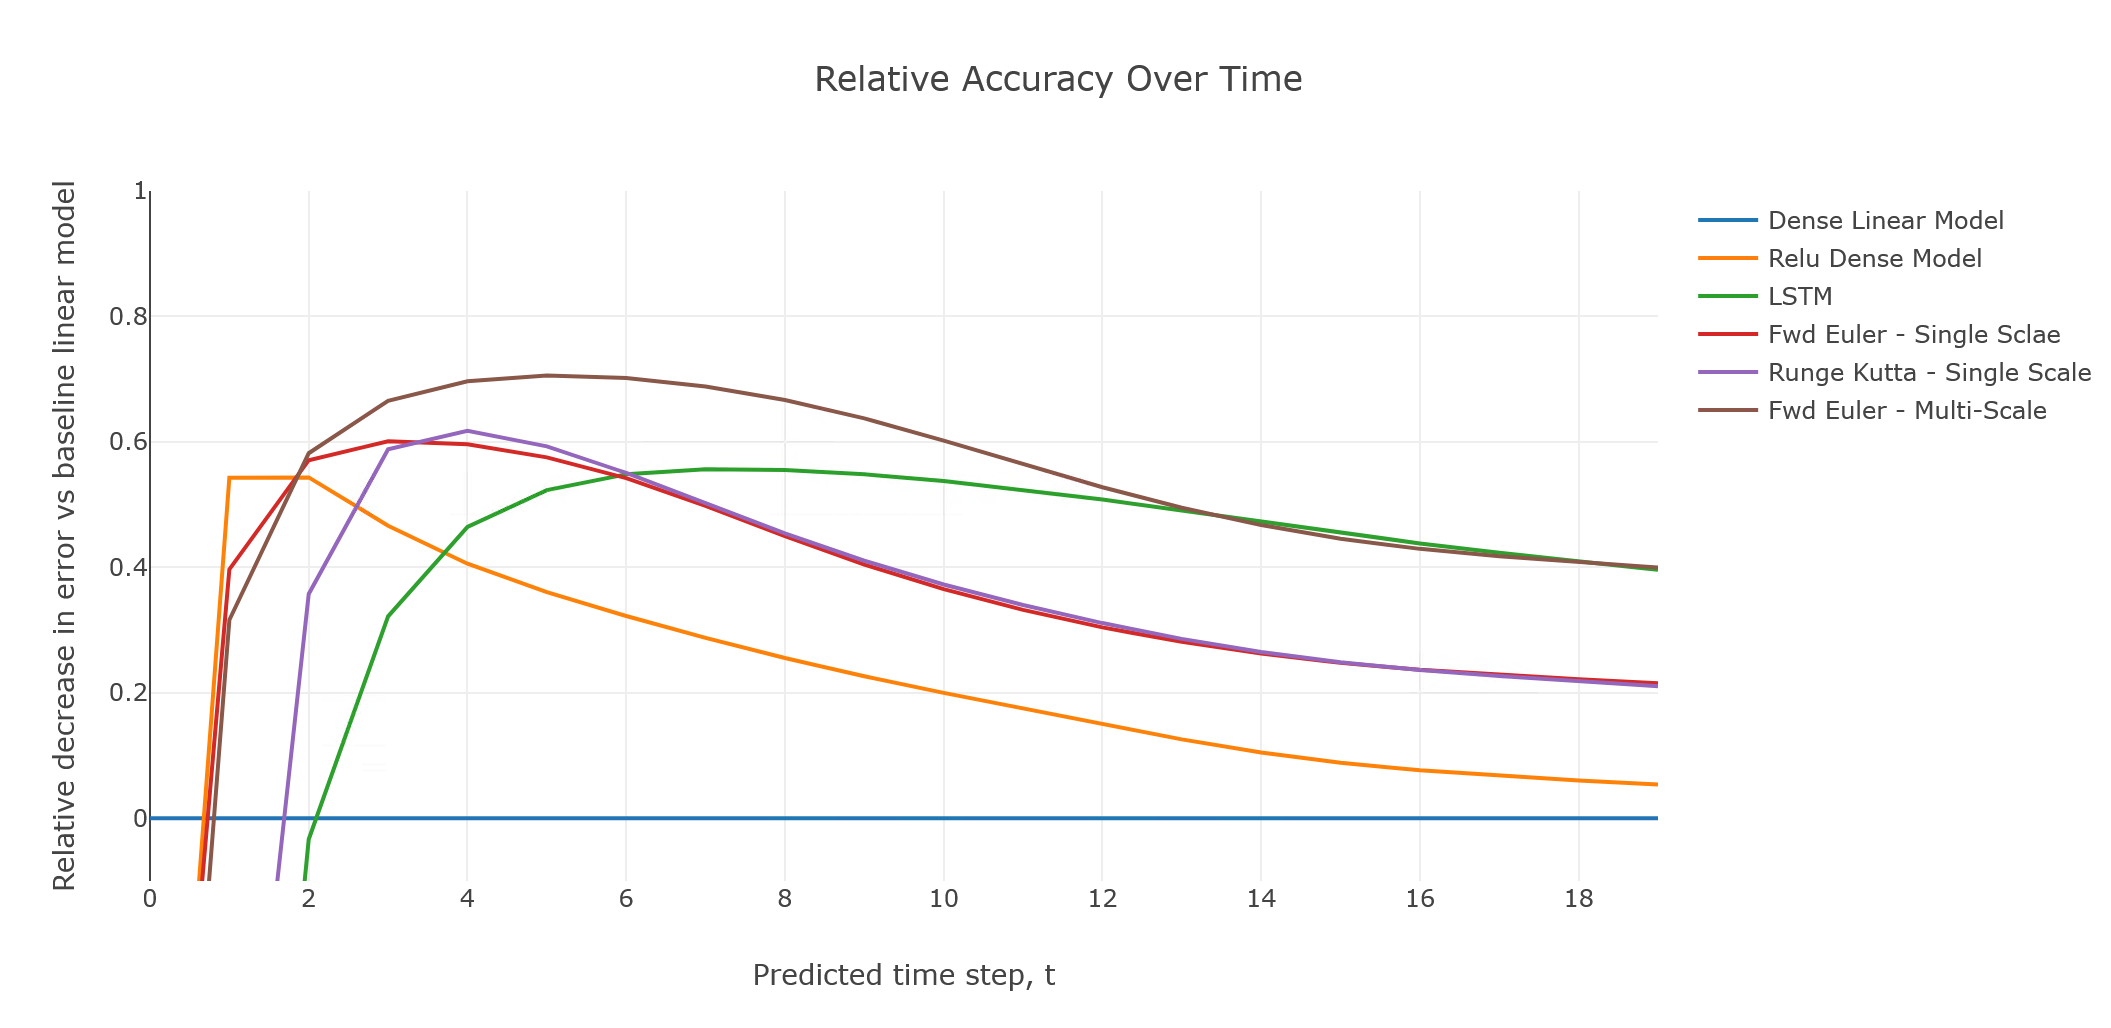
\includegraphics[width=0.95\linewidth]{image_preview}
	%	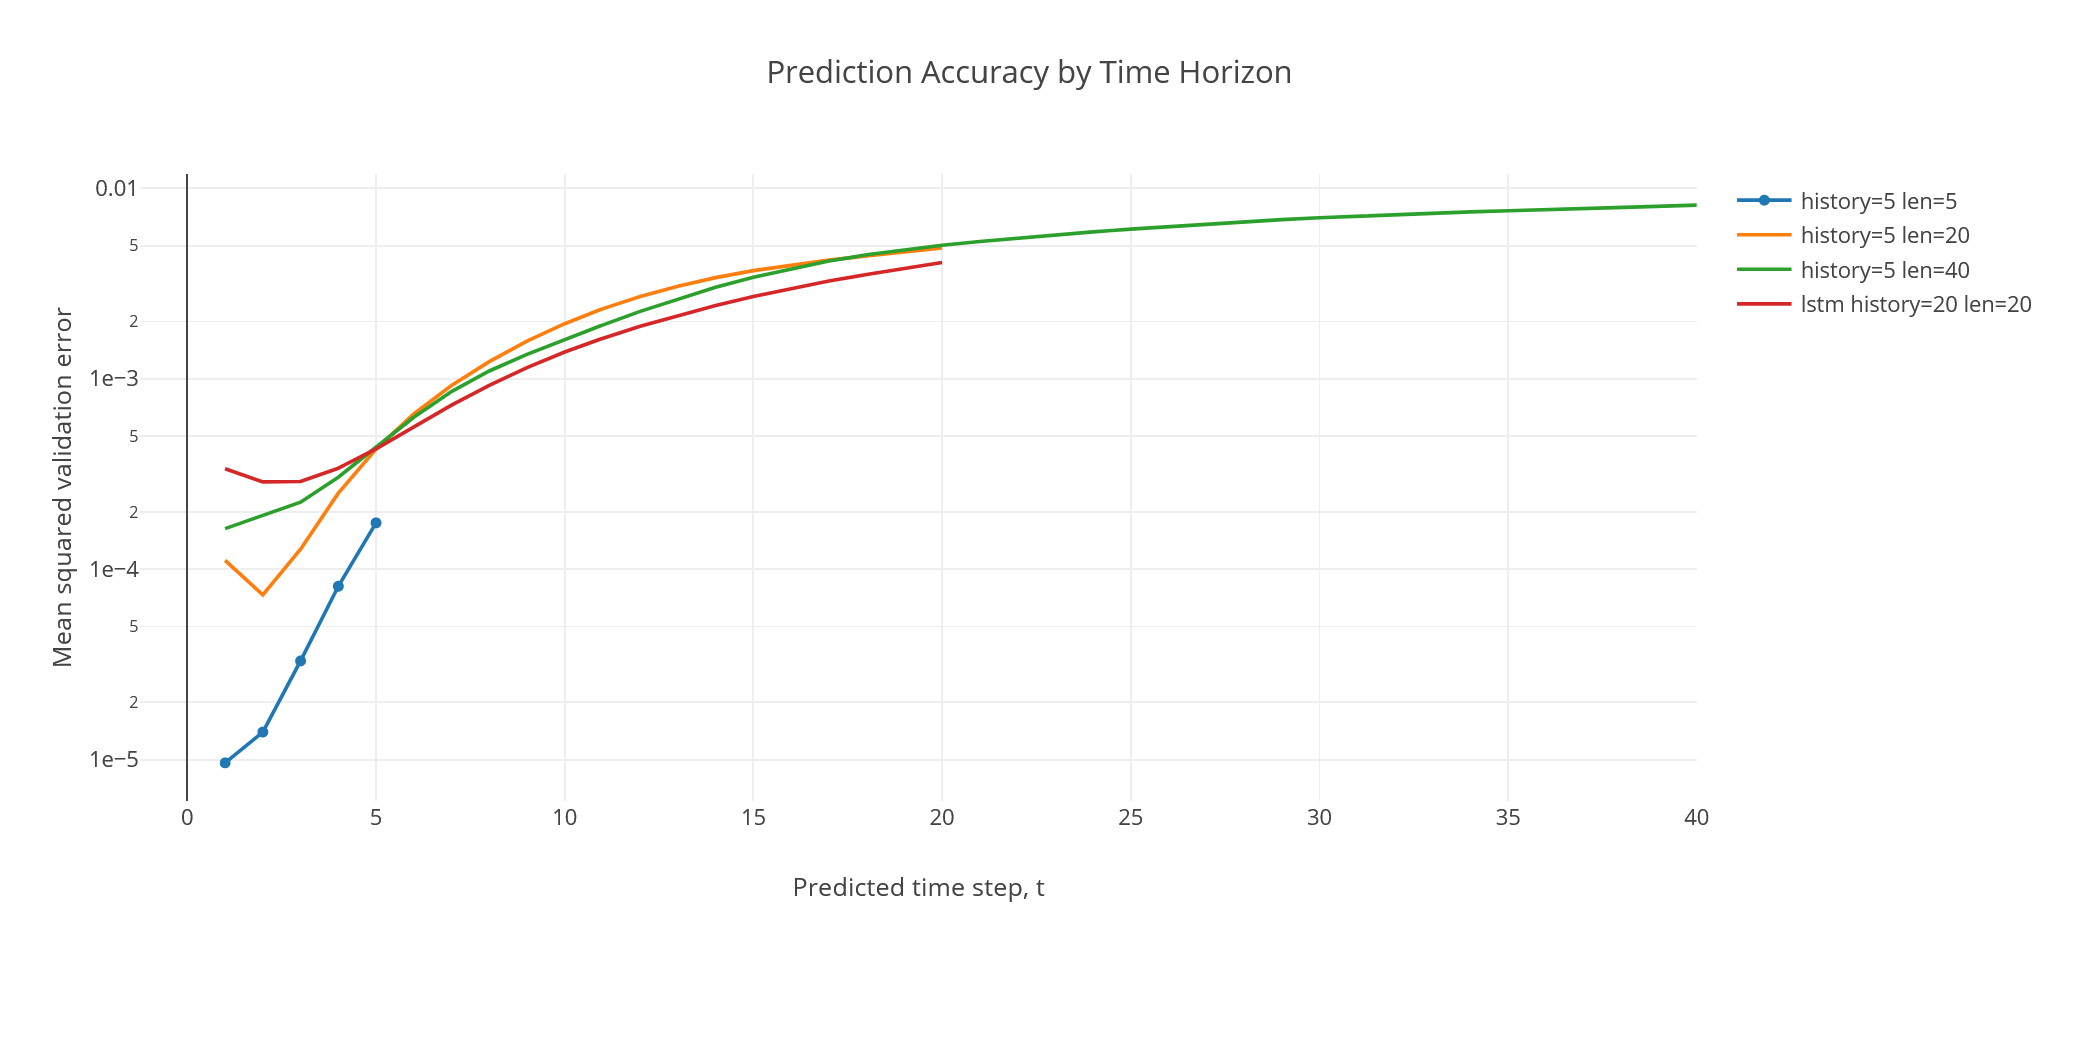
\includegraphics[width=0.9\linewidth]{pde_perf_linear}
	\caption{\small Relative baseline performance of various architectures as compared to a fully connected linear model (6.25 million parameters). A relative error decrease of 1.0 represents perfect prediction for a given time-step. Note the advantage of the foward-Euler multi-scale architecture across most time-steps.}
	\label{fig:pdeperf}
\end{figure}	

\begin{figure}
	\centering
	
\includegraphics[width=0.95\linewidth]{high_frequency_noise}
	%	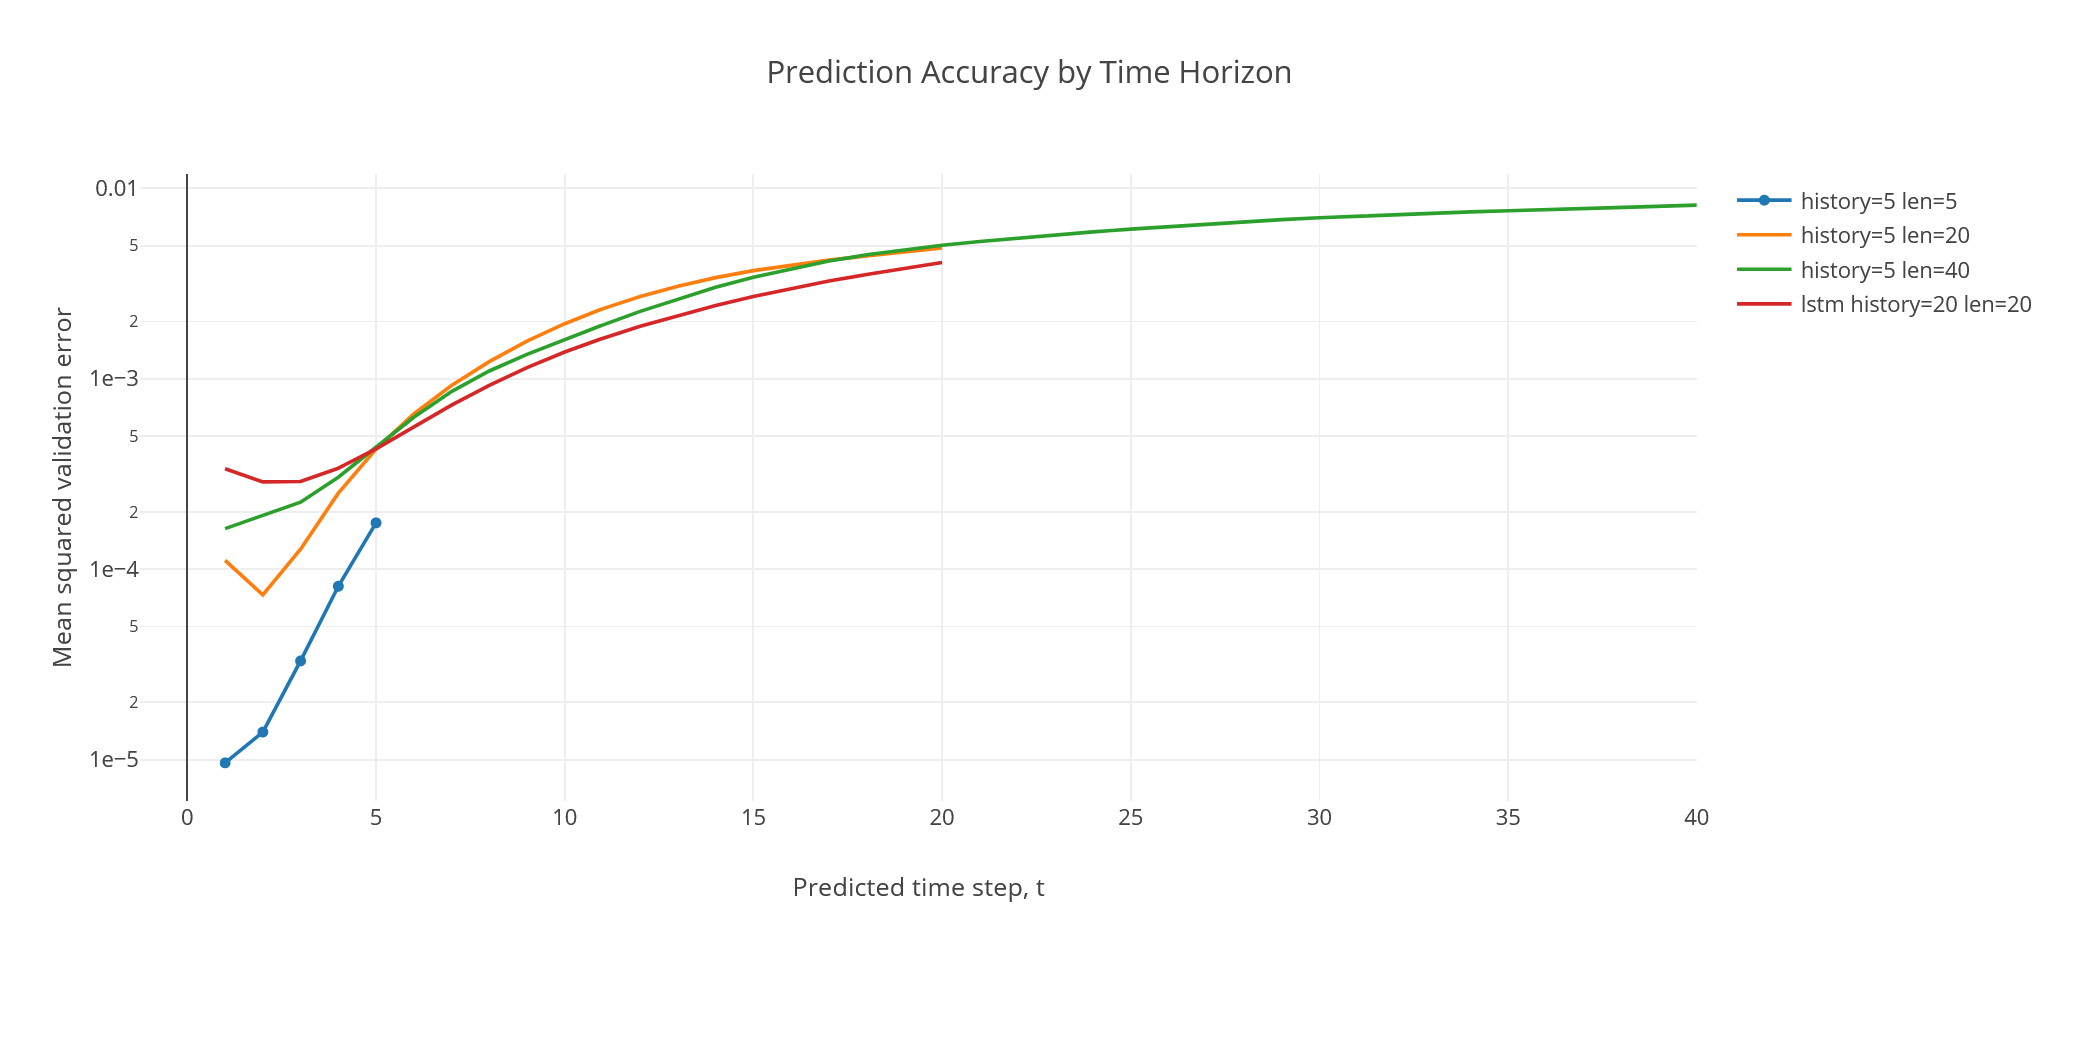
\includegraphics[width=0.9\linewidth]{pde_perf_linear}
	\caption{\small Relative baseline performance of various architectures as compared to a fully connected linear model (6.25 million parameters). A relative error decrease of 1.0 represents perfect prediction for a given time-step. Note the advantage of the foward-Euler multi-scale architecture across most time-steps.}
	\label{fig:pdeperf}
\end{figure}	

\begin{figure}

	\centering
	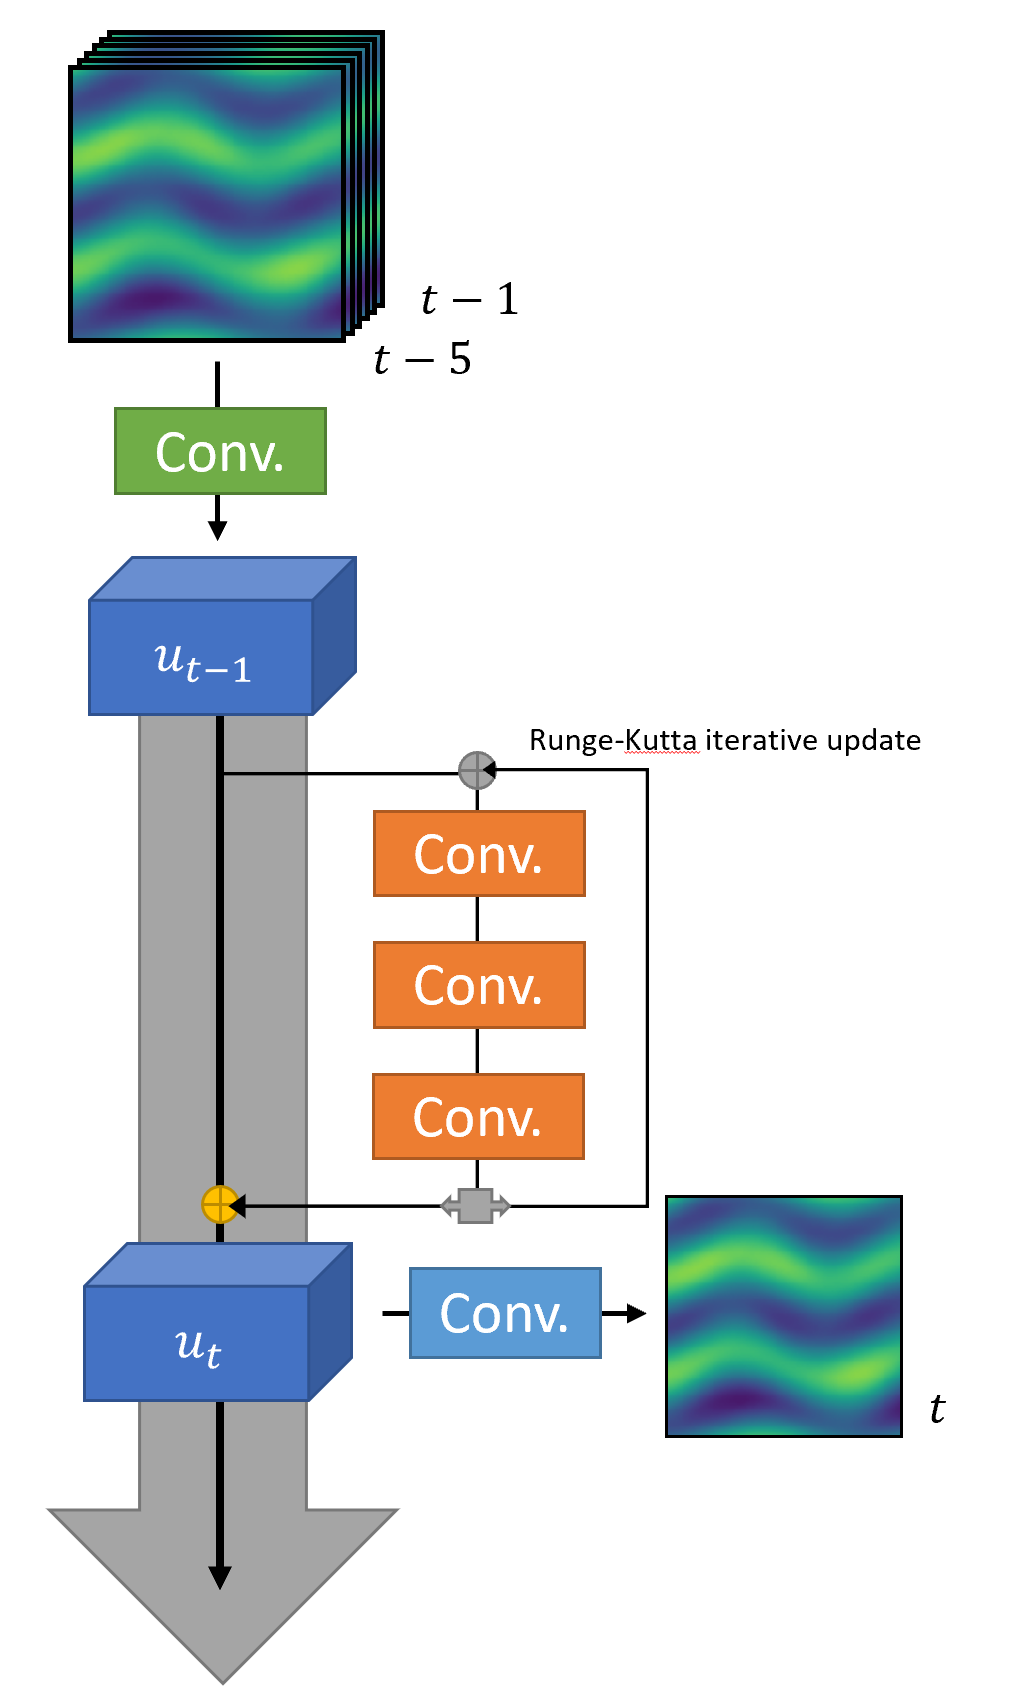
\includegraphics[width=2.5in]{pde_arch_rk4}
	\caption{Illustration of the iterative Runge-Kutta architecture. The encoder $\phi(x)$ (shown in green) maps the input $x$ into the feature space $u_t$. Three sequential convolutional layers (shown in orange) are applied, using the activation from the previous time-step to calculate the next update as described in the RK4 method. This generates a more precise estimate of the dynamics, taking into account the curvature at the mid-point as well as either end rather than the one-sided explicit update used by the  Euler method. The learned dynamics update $f(u_t)$ is then summed with $u_t$ (shown in yellow) to give $u_{t+1}$. At each time step $t$, the feature vector $u_t$ is decoded by $\theta(u_t)$ (as shown in light blue) predicting the vorticity at time $t$, $x_t$. }
	\label{fig:arch_rk4}

\end{figure}


Previously, we developed a forward Euler inspired network architecture that rivaled the performance of the previous LSTM based architectures. We also demonstrated the similarity of this architecture to numeric solvers for partially differential equations (PDEs).

To evaluate new models in a standard way, we first establish a baseline performance using a fully connected linear network, and introduce a relative baseline performance metric, where $\sigma$ represents the mean squared error of the model for a given time-step t.
$$RBP =  \frac{1}{n}\sum_{t=1}^{n}\frac{\sigma_{baseline} - \sigma_{model}}{ \sigma_{baseline}}$$ 

This gives us a score of 1 for models that perfectly explain the test data, and a score of 0 for models as good as a linear model (negative scores indicate models perform worse than the fully connected linear baseline).

In this period we significantly increased the performance of model architectures discovering new learning procedures and model architectures. As compared to our previous LSTM models with relative baseline performance (RBP) of 0.358, further improvements to training procedures (hypothesis 2) increased the RBP of the previously discovered forward Euler architecture to 0.386. 
Furthermore, by introducing multi-scale networks (hypothesis 1,) we see a 28.7\% reduction in mean squared error over 20 time steps resulting in a new architecture with an RBP of 0.548. Finally, we introduce a curriculum learning approach (hypothesis 3) that leverages different scales to train architectures that were previously impossible to train given their sensitivity to co-variate shifts. 


\subsection{Hypothesis 1 - Constraining Boundary Conditions}

Previously we found using convolutions at varying scales to increase the fidelity of the dynamics model while maintaining the symmetry-constrained properties of a convolutional architecture. We evaluate the performance of the forward-Euler architecture (illustrated in figure \ref{fig:arch})with and without multi-scale features, figure \ref{fig:abs_perf_new}, and see significant improvement in relative performance resulting in a $28.7\%$ decrease in mean squared error as compared to the previous best architecture. 

\subsubsection{What was to be tested? What was the expected outcome prior to testing?}
	We test the addition of convolutional features at different scales to learn the problem dynamics more accurately. The resulting architecture is illustrated in figure \ref{fig:arch_multi}. Previous architectures used only a single scale for convolutional features meaning the network had access to only local information. By adding multiple scales to the dynamics update we hope to enable the network to learn to use both local and global features in the region to predict more accurately.


\subsubsection{High-level summary of main results.}
	We see strong performance gains by the addition of the additional scales. As shown in figure \ref{fig:pdeperf}, for the multi-scale architecture prediction is accurate over both the short-term and long-term predictions, beating LSTM based methods in short-term prediction.  


\subsubsection{Discuss relevance to project and DARPA concerns.}
	In numeric PDE solvers, choosing the proper simulation scale can dramatically effect the accuracy of simulations even for known PDEs. Given the increase in performance we see that with the addition of multi-scale convolutional layers, networks learn the proper scale for accurate prediction dynamically. This results in networks that are general and adapt well to new problems.


\subsection{Hypothesis 2 - Iterative approximation methods}

 We implemented the fourth-order Runge-Kutta method by iteratively sampling the dynamics model (shown in orange in figure \ref{fig:arch_rk4}) to obtain a more accurate estimate of the next time-step, $u_t$. In testing this method directly on single-scale architectures, performance of the model both computationally and numerically were reduced. Further investigation is needed to determine if a different formulation of the loss function could be effective in lowering compounding error and enabling better long-term predictions. 

\subsubsection{What was to be tested? What was the expected outcome prior to testing?}
	Given the similarity between our network architecture and the update step used by forward-Euler approximations, we proposed integrating techniques effective in reducing the compounding error approximate solutions for ordinary differential equations. Using the existing architecture to predict the next point, taking a small gradient step in that direction, then updating our prediction. We expected this method to increase the accuracy of the learned model by adjusting for local curvature. 


\subsubsection{High-level summary of main results.}
	The fourth order Runge-Kutta method as applied (see figure \ref{fig:arch_rk4}) did not improve performance and increased the computational requirements during training. Future work is needed to explore if this method could be effective if introduced into the curriculum learning approach outlined in hypothesis 3. Runge-Kutta as tested in these experiments reduces to an averaging of an iterative procedure which may be intractable given the non-linear nature of the model architecture.


\subsubsection{Discuss relevance to project and DARPA concerns.}
	If successfully applied, iterative methods can leverage traditional understanding of time-discretized ordinary differential equations to improve the accuracy of models without requiring additional training steps or more training data.


\subsection{Hypothesis 3 - Scale adapted curriculum learning}

In experiments concerning hypothesis 2, we experienced an explosion of gradient updates - where small shifts in network parameters were amplified making learning impossible for these interesting network formulations. To address this issue, we proposed a dynamic adjustment of the prediction horizon while training, forming a curriculum-learning approach where simpler short-term dynamics are learned before introducing longer-term dynamics which have higher sensitivity to rapid shifts in network dynamics. This approach was effective in enabling experiments on iterative descritized approximation methods.


\subsubsection{What was to be tested? What was the expected outcome prior to testing?}
	We evaluate models over increasingly distant time-steps to determine if this procedure regularized the network and prevented explosion of gradients. Given the short reward horizon we expected this method to decrease the variability of gradient updates and allow for stable gradient decent.


\subsubsection{High-level summary of main results.}
This approach expanded the domain of model architectures to experiment on and increased the stability of training allowing for more aggressive gradient steps as well as reducing the amount of data required for early training steps.

\subsubsection{Discuss relevance to project and DARPA concerns.}
By varying the prediction length early on, the decrease in computation dramatically speeds up training time and increases the stability of the learning procedure.
%========================================================================
\section{Achievements}

\subsection{Scientific Breakthroughs}

None

\subsection{Technology developments}

None

\subsection{Application results}

Predictive performance has demonstrated that despite the difficult problem of predicting chaotic systems, using scale-adapted and symmetry constrained architectural components are able to predict better than LSTM based architectures and significantly better then baseline linear models.

\subsection{Transitions achieved}

None

%========================================================================
\section{Lessons Learned}


\noindent Problems encountered/risks that occurred, and corresponding solutions/mitigations

None

\noindent Open Issues

None

%========================================================================
\section{Next Steps}

\noindent We would like to further refine the multi-scale architecture, specifically testing networks that include additional scales of convolutional features.


\noindent Current results reflect only one ground truth scale. Testing with super-sampling and sub-sampling to establish scale invariance would be an interesting exploration for the current model architecture.

\noindent When used naively, fourth order Runge-Kutta did not improve the performance of the model. Instead of using Runke-Kutta directly on the same $f(u_t)$ we would like to explore learning separate iterative midpoints to use in the dynamics update step.  


%========================================================================
\section{Technical details}

\begin{figure}
	\begin{minipage}[c]{0.49\textwidth}
		\centering
		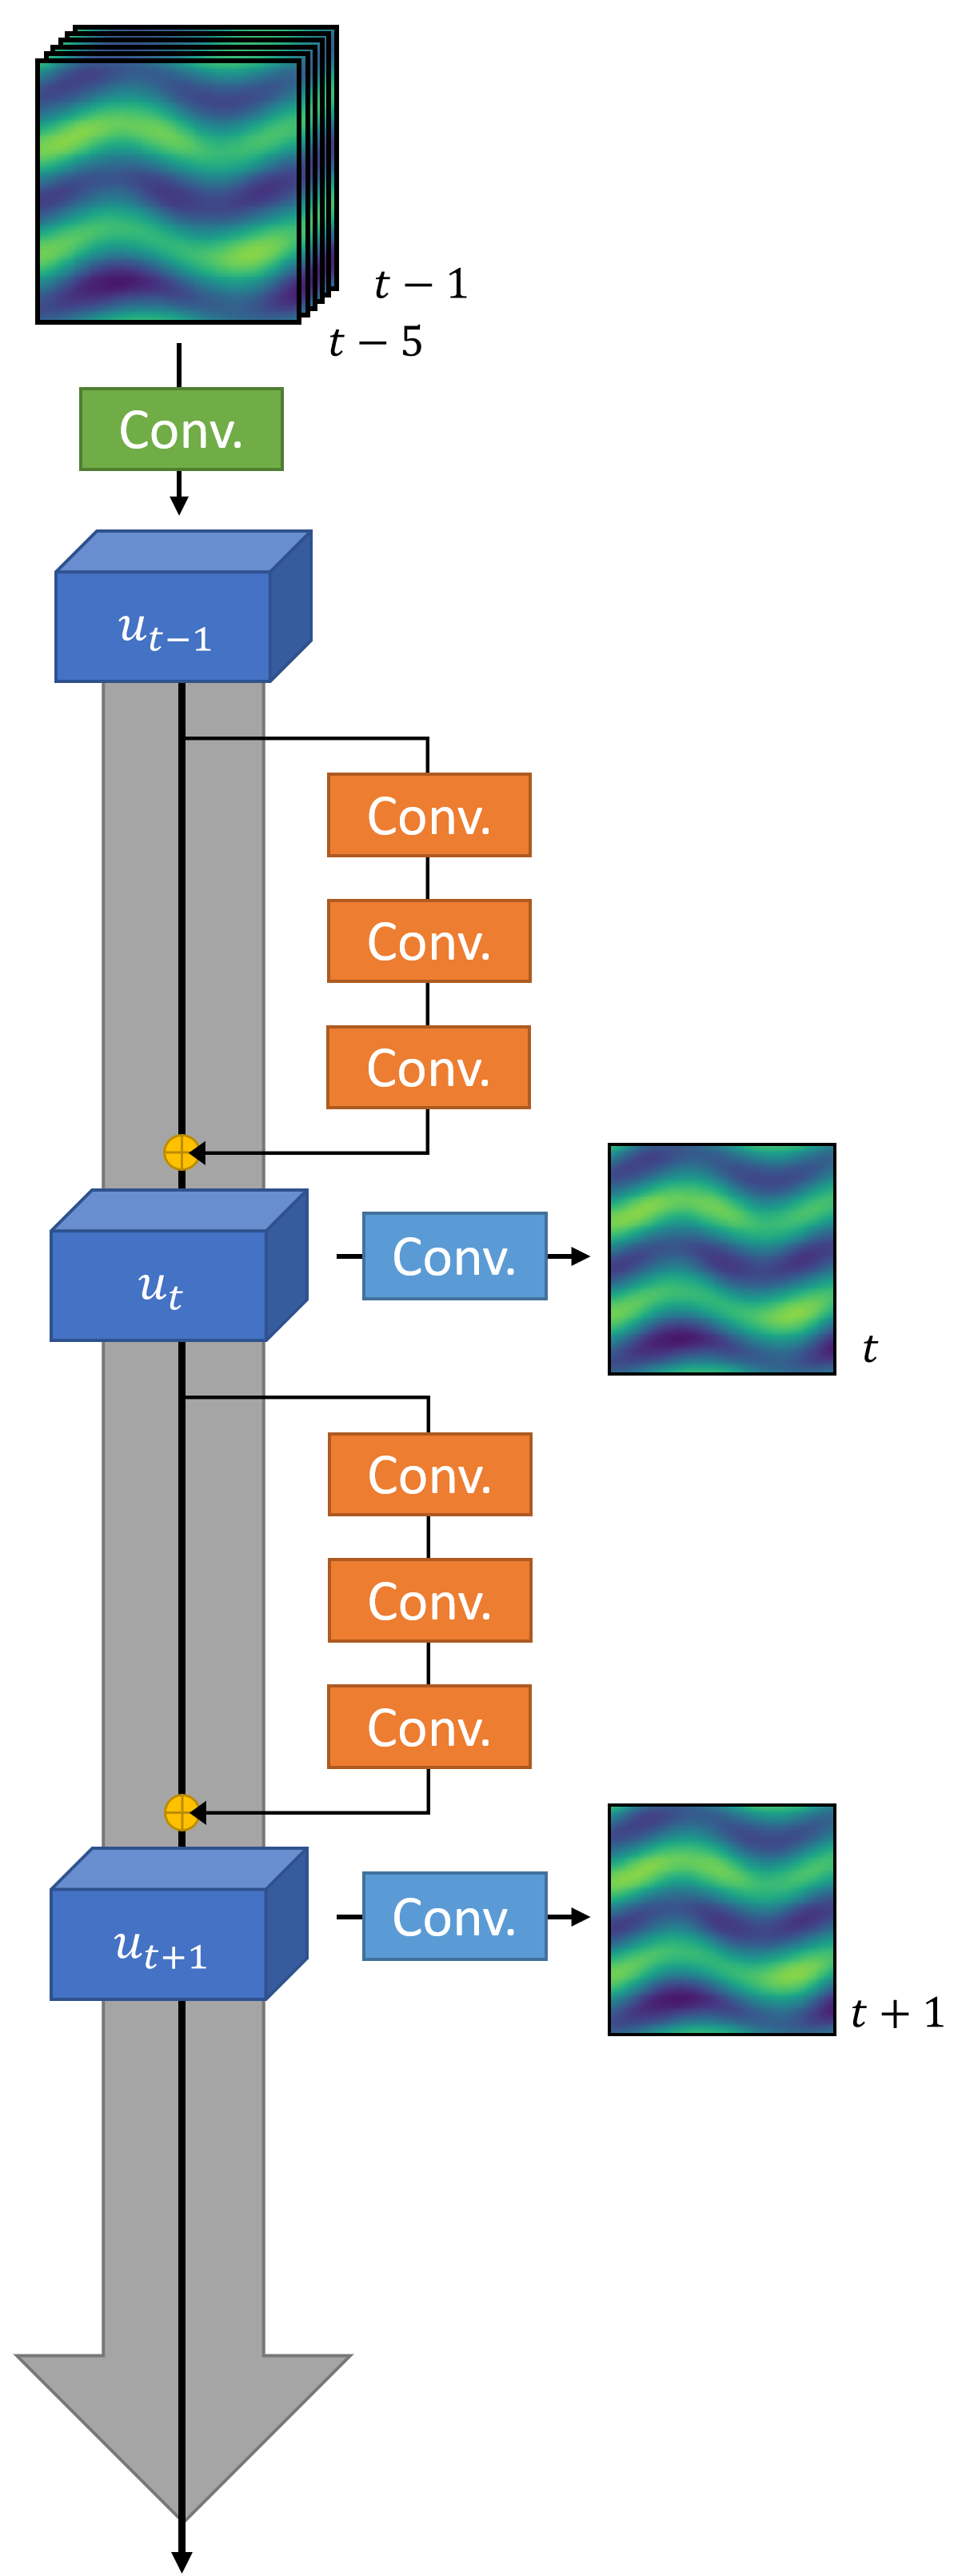
\includegraphics[width=2.5in]{pde_arch}
		\caption{Illustration of the previous forward Euler architecture. The encoder $\phi(x)$ (shown in green) maps the input into the feature space. Three convolutional layers (shown in orange) are used to approximate $f(u_t)$ and summed with $u_t$ (shown in yellow) to give $u_{t+1}$ as outlined in equation \ref{eqn:ode}. At each step, the feature vector $u_t$ is decoded by $\theta(u_t)$ (as shown in light blue) predicting $x_t$.}
		\label{fig:arch}

	\end{minipage}
	\begin{minipage}[c]{0.49\textwidth}
		\centering
		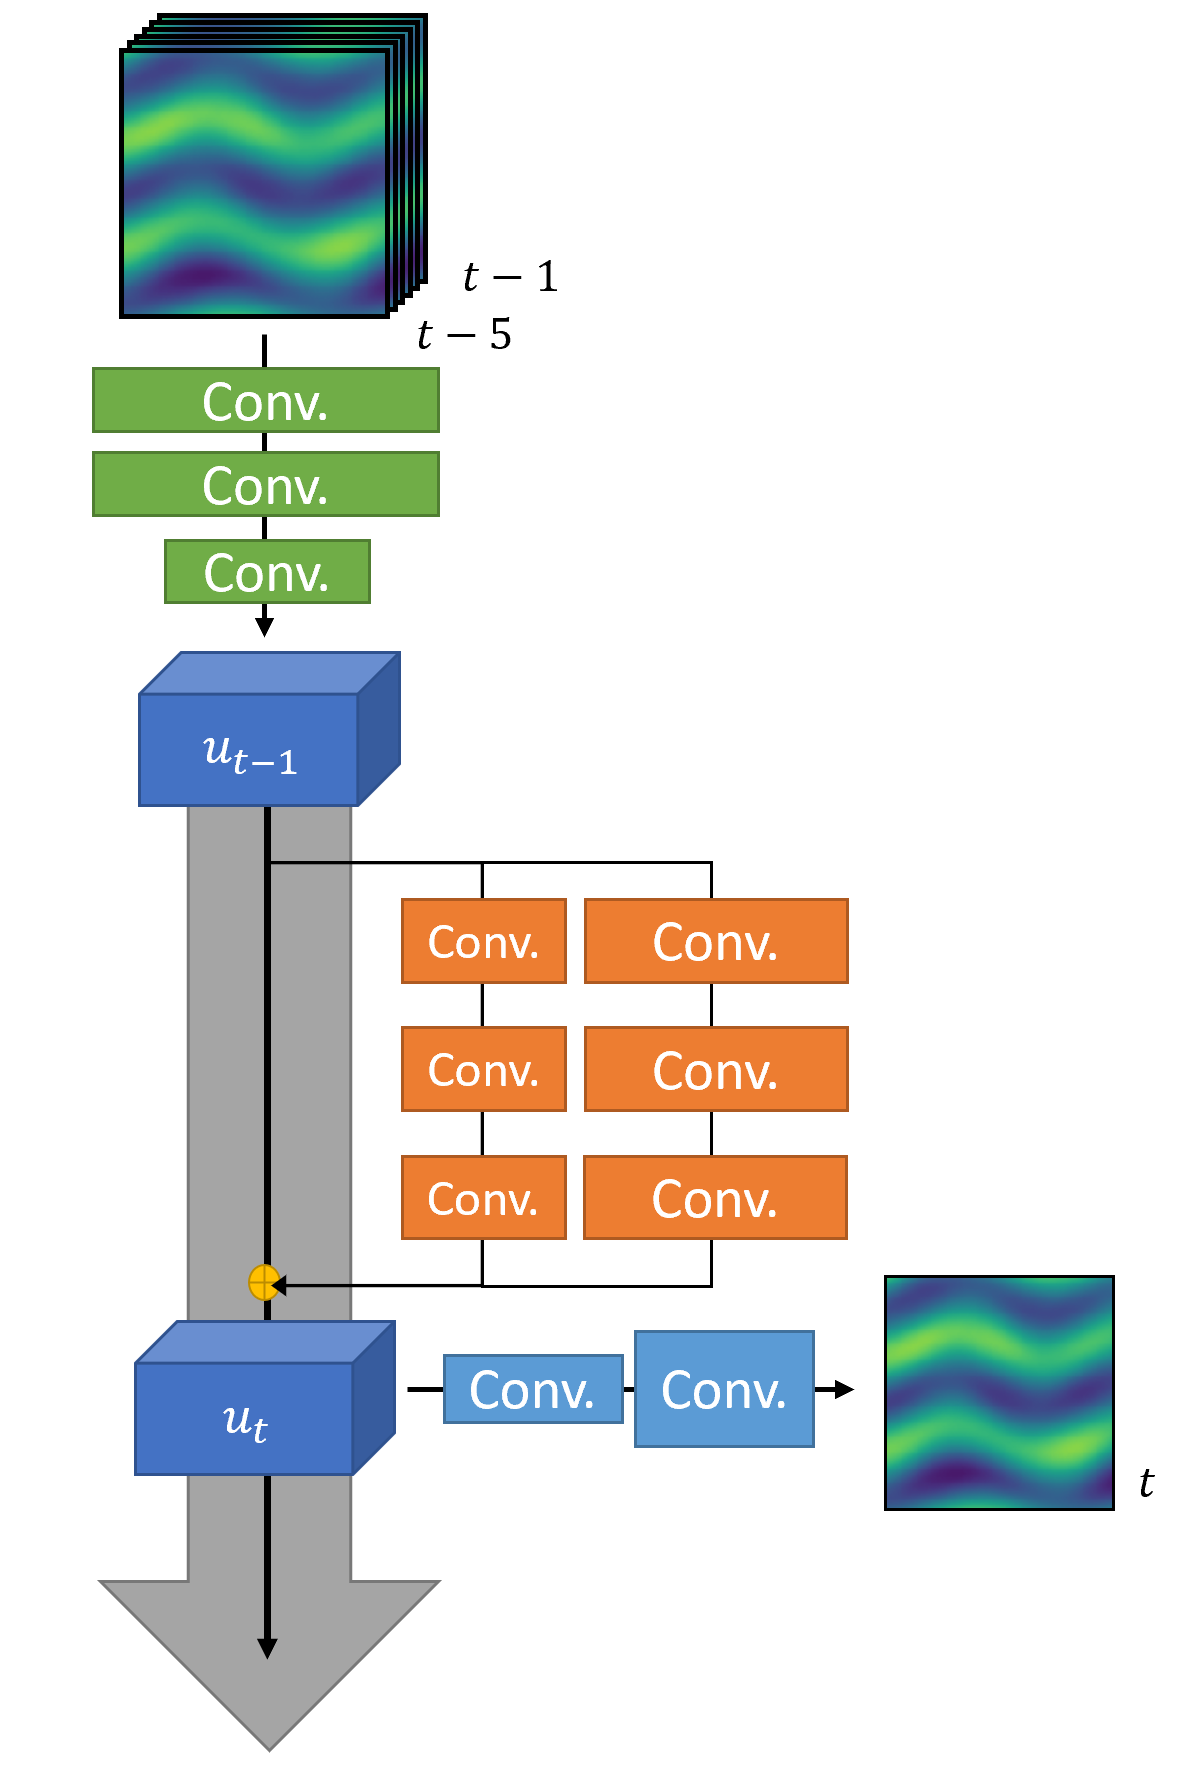
\includegraphics[width=2.75in]{pde_arch_multi}
		\caption{Illustration of the multi-scale forward Euler architecture. The
		dynamics $f(u_t)$ are enriched with filters at different scales (shown in orange). Additionally, the encoder $\phi(x)$ reduces the dimensionality of the input image by a factor of 4 in the encoding step $\phi(x)$ to increase the receptive field of the dynamics update calculation, $f(u_t)$. }
		\label{fig:arch_multi}
	\end{minipage}
\end{figure}



\subsection{Formulating Multi-Scale Architecture}

Consider learning a PDE of the form $u_t = f(u)$. The simplest approximation of $u_t = f(u)$ is to discretize the time derivative $u_t$ by $\frac{u_{n+1} - u_n}{\bigtriangleup t}$ and approximate the right hand side by $f(u_n)$. This leads to the forward Euler scheme  

$$u_{n+1} = u_n + \bigtriangleup t f(u_n) \label{eqn:ode} $$

where $f(u_n)$ is learned by a deep neural network. Instead of learning the dynamics of the system directly, we use a learned feature representation $u_n$ composed of linear convolutions of the input history. This avoids the need for approximating the local partial derivatives of the system and instead allows the network to learn the optimal feature representation.


Let $x$ represent h patches of history $x = [x_{t-h}, ..., x_{t-1}]$ and y represent the target sequence $y = 
[x_{t}, x_{t+1},...,x_{t+l-1}]$.  We learn an encoder, $\phi(x) = u_0$, a decoder $\theta(u_n) = \hat{x}_n$ as well as a dynamics model $f(u_n)$ from equation \ref{eqn:ode}.  

In the new multi-scale architecture shown in figure \ref{fig:arch_multi} we utilize a feature space of dimension m = 64, and reduce the spacial dimensions of the image patch by a factor of 4 therefore, $u_n \in \R^{64, 25, 25}$. 
In constructing the multi-scale element of $f(u_n)$, the first layer of each scale reduces the feature space (64) down to $\frac{1}{num\_scales}$ features (32 as implemented in the multi-scale architecture outlined in figure \ref{fig:arch_multi}). Each scale is then computed in parallel and then the activations are concatenated. This allows each scale to signal other scales while lowering the number of learnable parameters as show to be successful in [F. Iandola et al. 2016]. Finally, the decoder $\theta(u_n)$ uses a de-convolution of size 2 to increase the spacial dimension of the embedded dynamics $u_n$ to 50x50x8 and a final linear convolution smooths the output of the network.

\begin{figure}
	\centering
	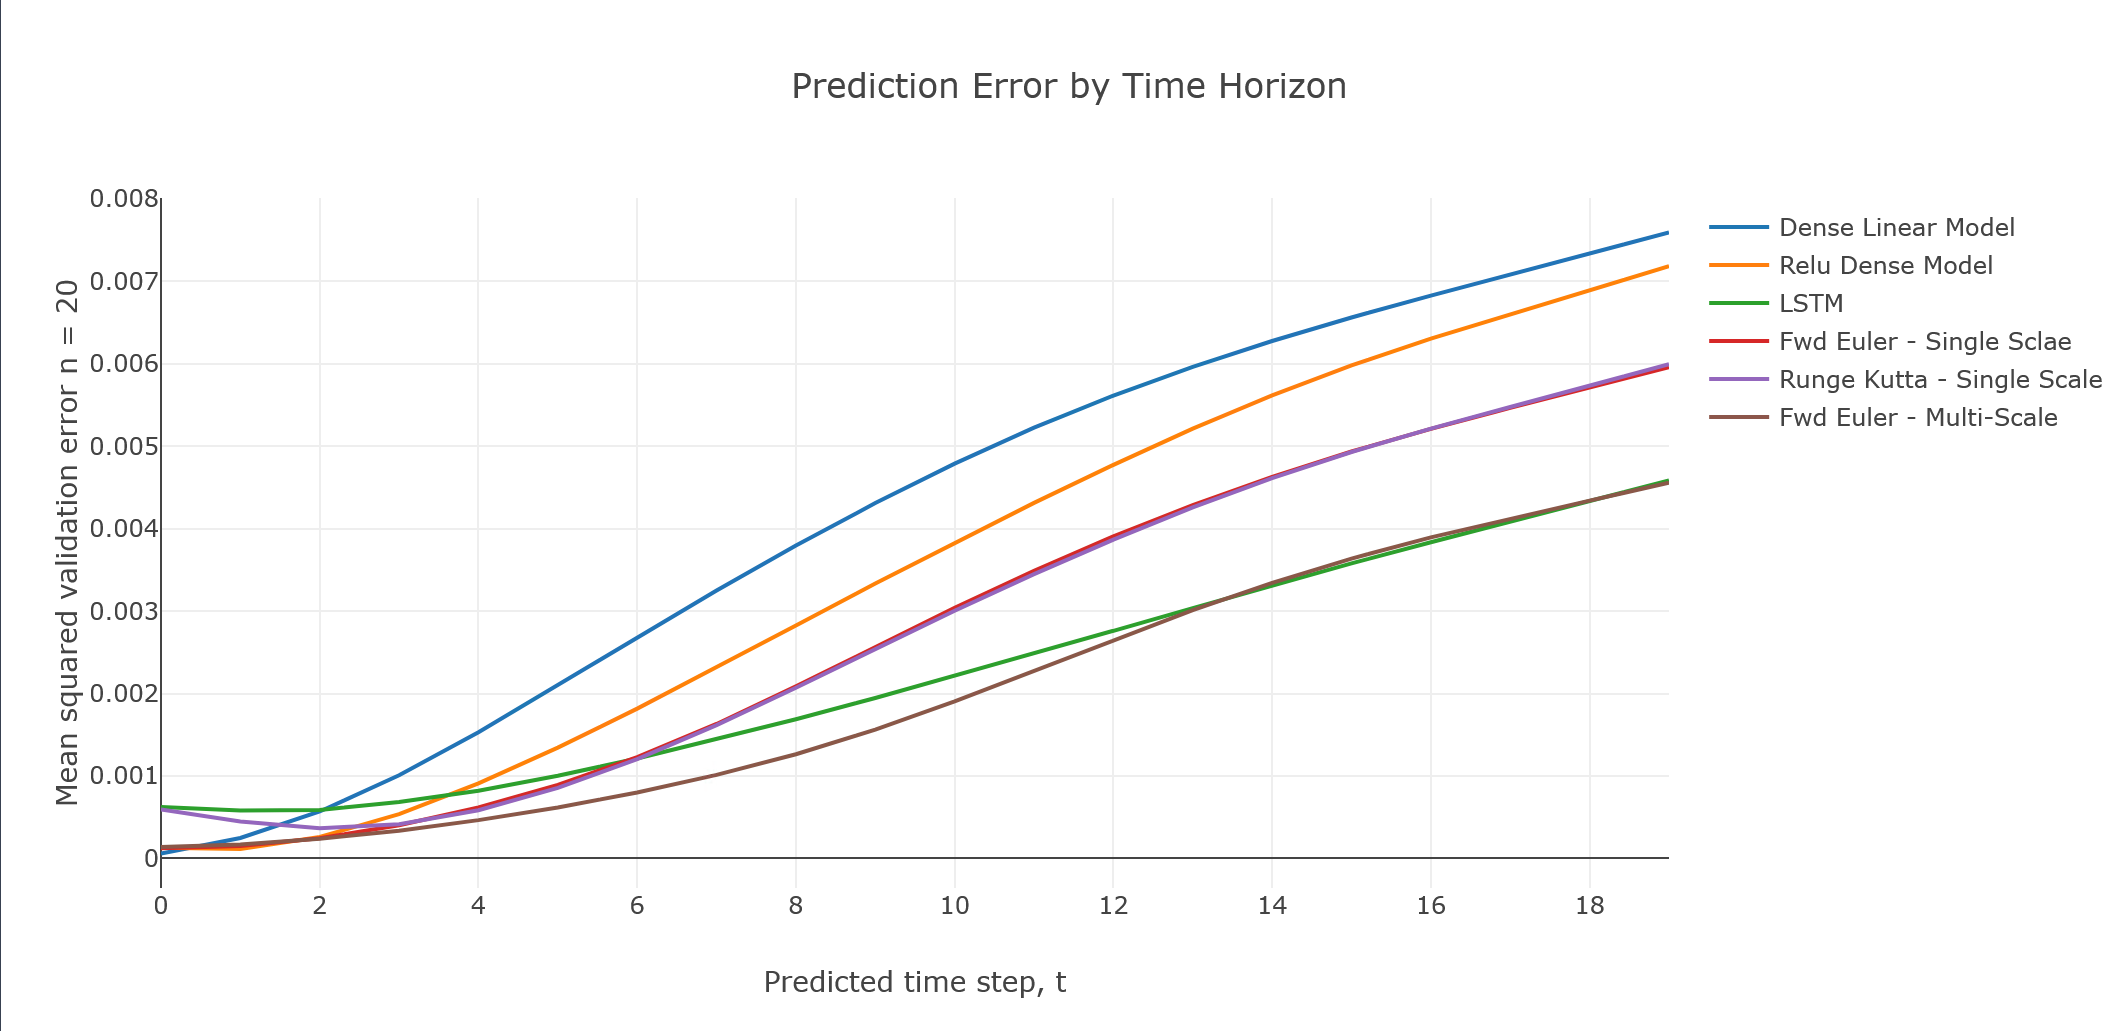
\includegraphics[width=0.95\linewidth]{abs_perf_new}
%	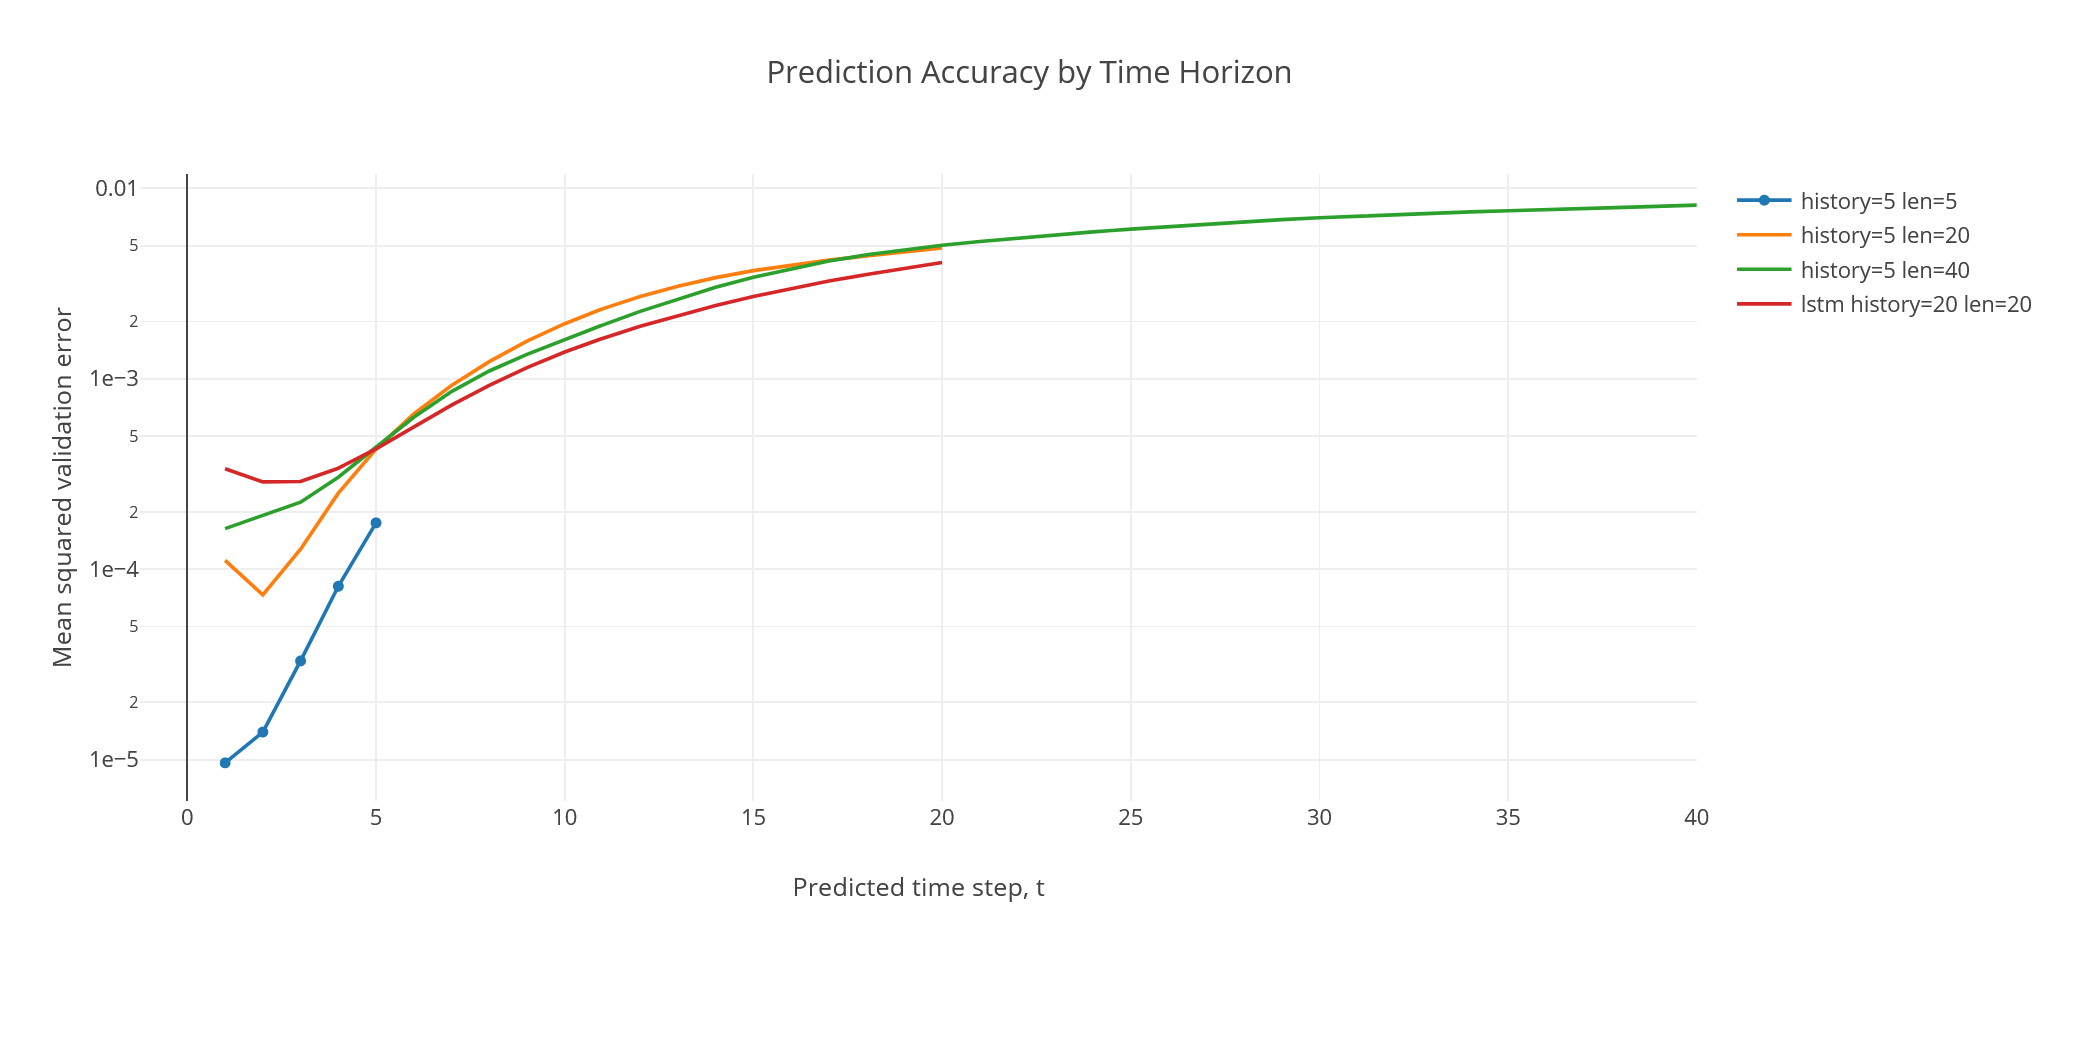
\includegraphics[width=0.9\linewidth]{pde_perf_linear}
	\caption{\small Relative baseline performance of various architectures. Note the advantage of the multi-scale architecture across most time-steps.}
	\label{fig:abs_perf_new}
\end{figure}


\subsection{Scale adapted curriculum learning}
Implementing multi-scale curriculum learning simple anneals the prediction horizon during training. By loading the model weights from previous runs, we start training the model to predict 2 time-steps into the future, increasing the prediction horizon by 2 until the desired prediction length is achieved. 
This simple modification both increased the number of training batches per second, and thus training speed, but also prevented the iterative R4 models from diverging during training which resulted because of the repeated application of model parameters causing the explosion of resultant gradients over long reward horizons.


\end{document}

